In Table~\ref{tab:typical}, we show typical values for the main dataset parameters. In Table~\ref{tab:dataset_desc}, we describe the main dataset parameters of the real datasets we used. In Figure~\ref{fig:memory_usage} we compare the memory usage of DetSRM, ProbSRM and FastSRM with different atlases as a function of the number of components used while performing the encoding experiment described in Section~\ref{reconstruction}. In Figure~\ref{fig:example_r2}, we show for the same experiment, the $R^2$ score per voxels averaged across cross validation folds. 


\begin{figure}
\centering
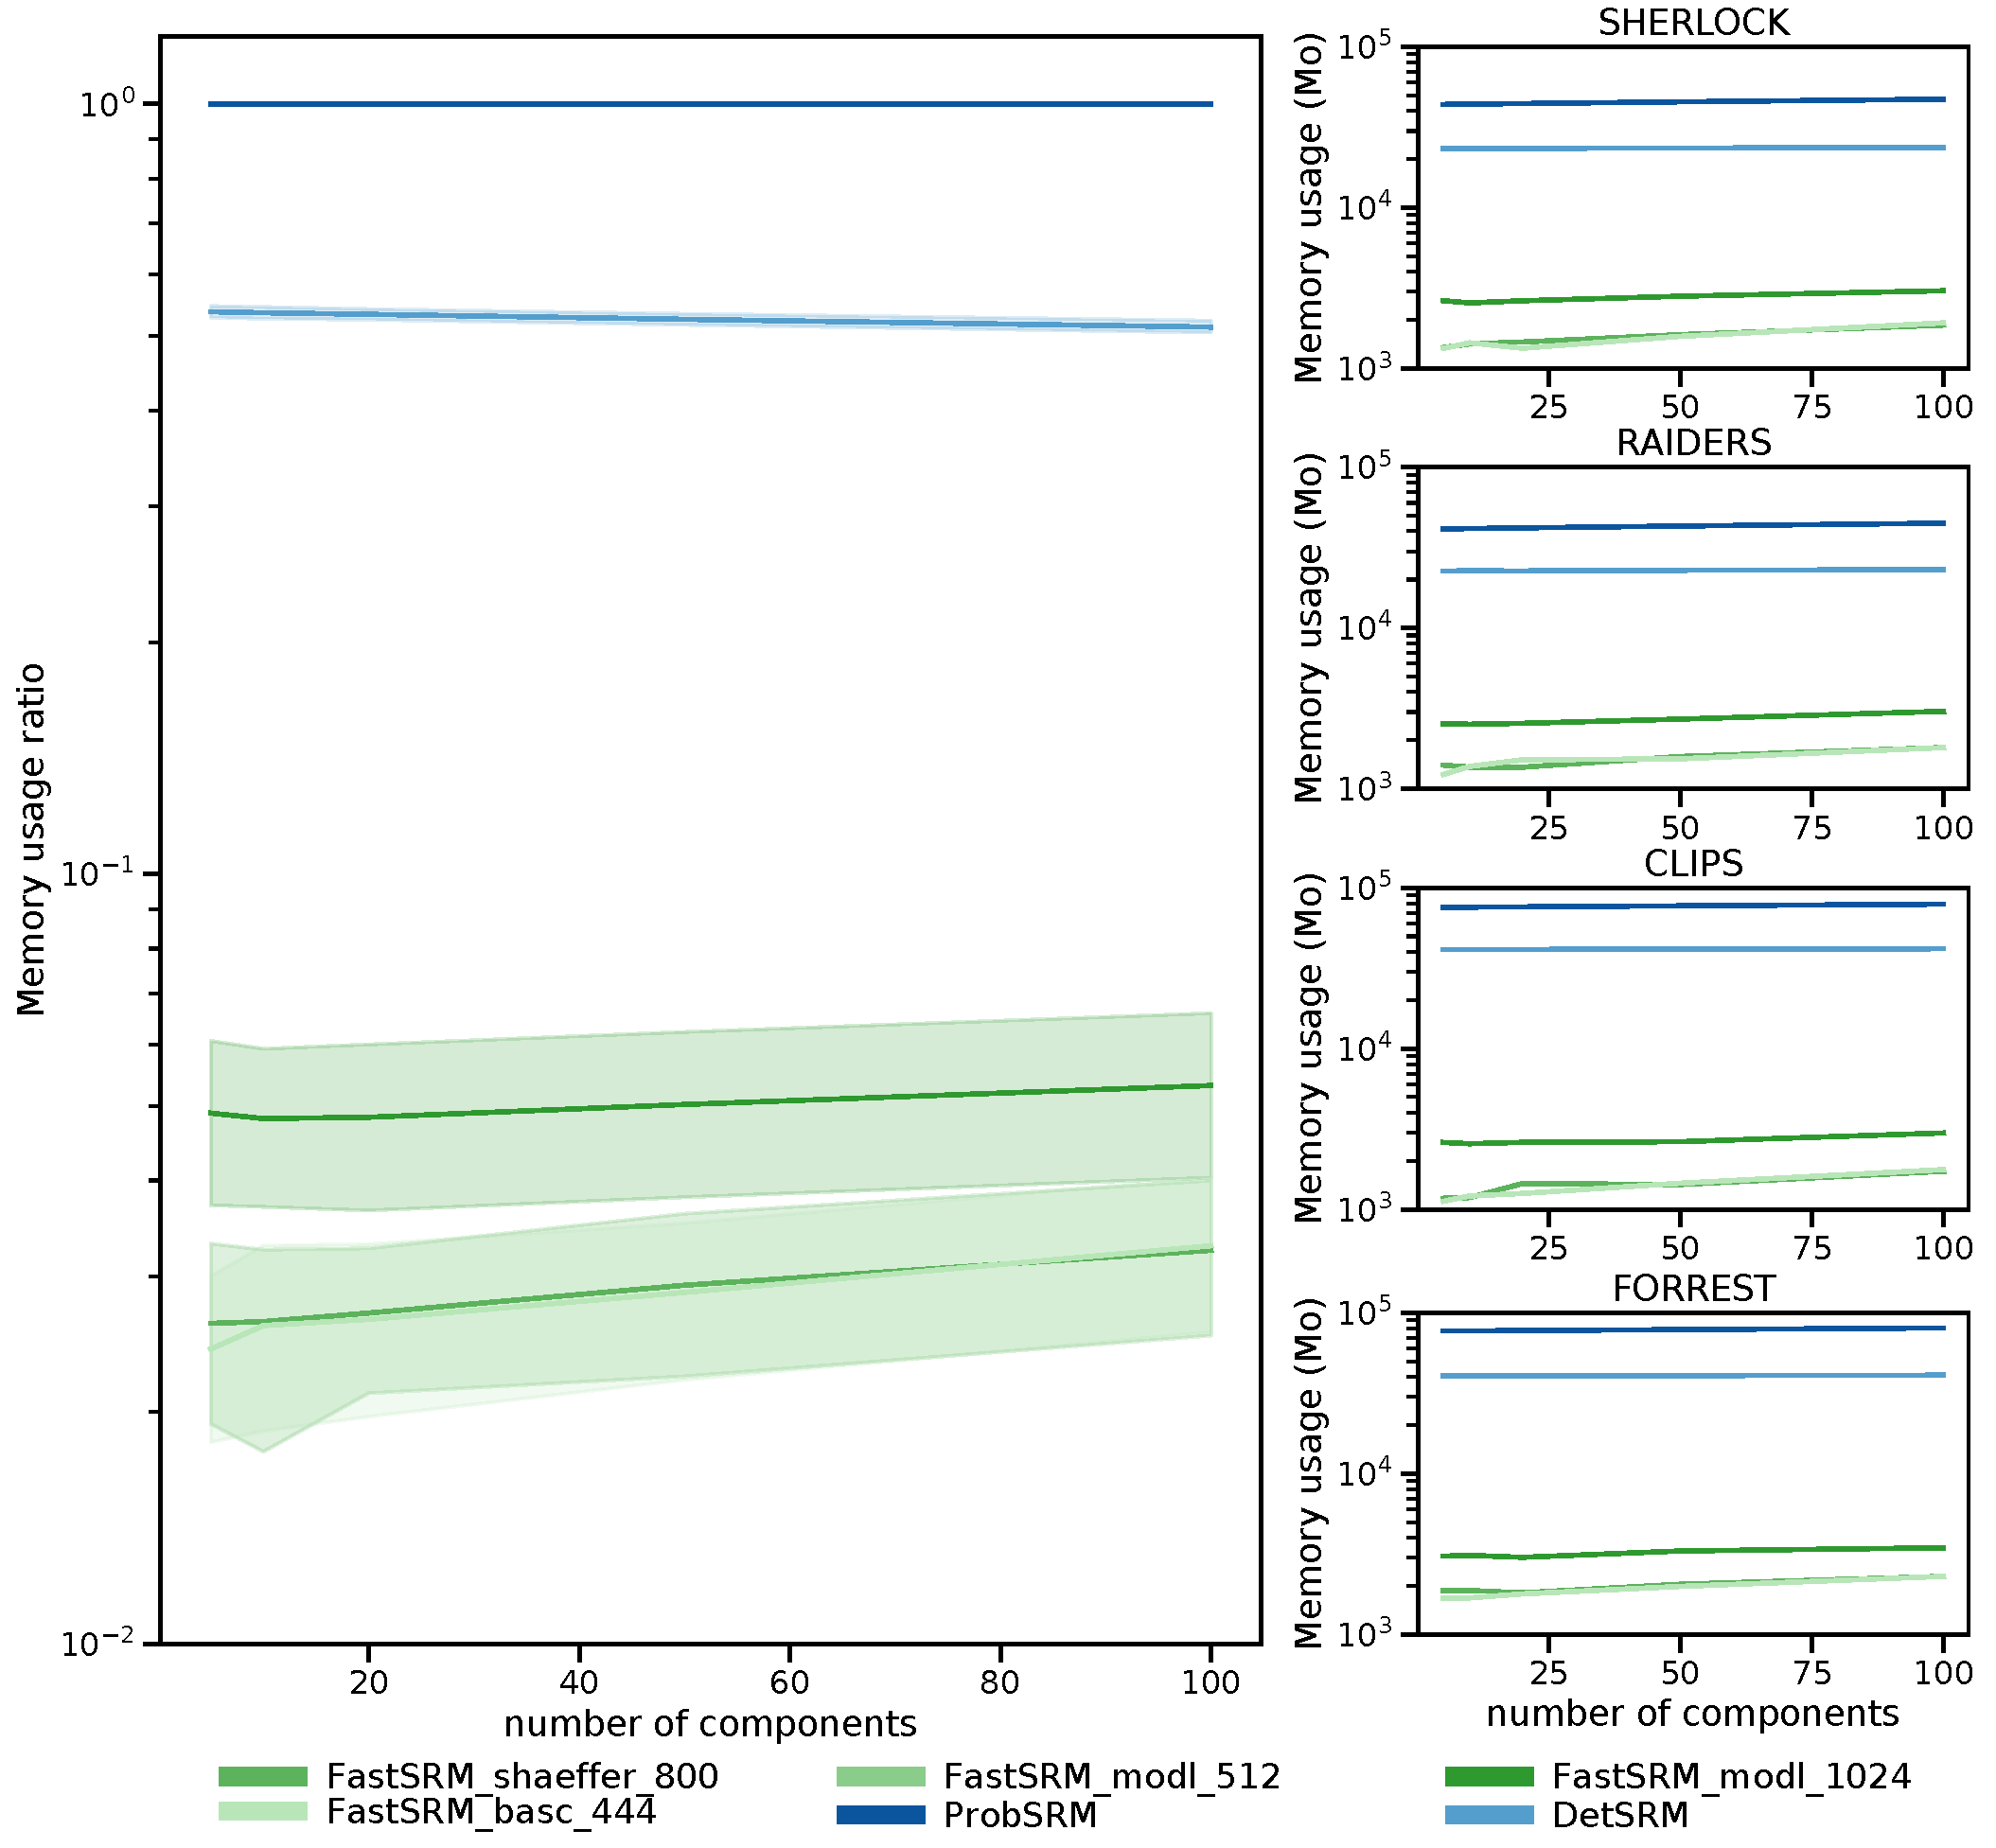
\includegraphics[scale=0.33]{figures/srm/memory_usage.pdf}
\caption{\textbf{Memory usage of FastSRM, ProbSRM and DetSRM} We compare the memory usage of DetSRM, ProbSRM and FastSRM with different atlases in function of the number of components used. Atlases tested are MODL with 512 and 1024 parcels, Basc with 444 parcels and Shaeffer with 800 parcels. Datasets tested are SHERLOCK, RAIDERS, CLIPS and FORREST.
\textbf{Left}: Memory usage (as a fraction of ProbSRM memory usage) averaged over the four datasets
\textbf{Right}: Memory usage (in Mo) for each of the four different datasets.
FastSRM with probabilistic atlases (MODL) is about 20x more memory efficient than ProbSRM and 40x with deterministic atlases (Basc, Shaeffer) making it possible to compute a shared response on a large dataset using a modern laptop.}
\label{fig:memory_usage}
\end{figure}


\begin{figure}
\centering
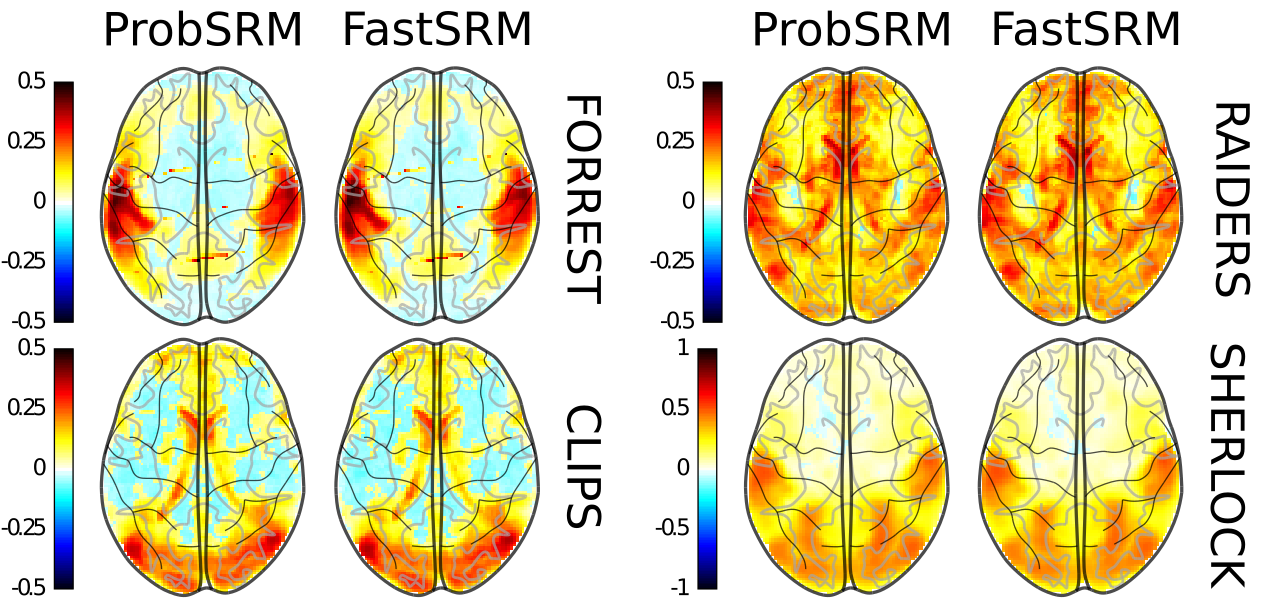
\includegraphics[scale=0.43]{figures/srm/mean_r2_reconstruction.png}
\caption{\textbf{fMRI reconstruction: $R^2$ score per voxels averaged across cross validation folds}: We benchmark ProbSRM and FastSRM using $20$ components on SHERLOCK, RAIDERS, CLIPS and FORREST datasets. An $R^2$ score of 1 means perfect reconstruction while 0 means that the model only predicts the mean of the voxel time-course.}
\label{fig:example_r2}
\end{figure}


\begin{table}
\centering
\begin{tabular}{c|c|c}
	Name of variable &  Notation & Typical value \\
	\hline
	Number of voxels & $v$ & [$10^5, 10^6$] \\
	Number of timeframes & $t$ & [$10^2, 10^3$] \\
	Number of runs & $m$ & $10$ \\
	Number of subjects & $n$ & [$10, 10^2$] \\
	Number of components & $k$ & [$10, 10^2$]
\end{tabular}
\caption{\textbf{Typical values for the main dataset parameters.}}
\label{tab:typical}
\end{table}
